\chapter{A Beautiful Theory}
\begin{aquote}{Murray Gell-Mann, Beauty and truth in physics, 2007}
    What is especially striking and remarkable is that in fundamental physics 
    a beautiful or elegant theory is more likely to be right 
    than a theory that is inelegant.
\end{aquote}

\section{The Standard Model}
Put simply, the Standard Model (Fig.~\ref{fig:standard_model}) attempts to describe, at the most fundamental level, what the universe is made of and how it operates. 
So far, the content of the model is as follows: the universe is made of fermions (quarks and leptons), and it operates through the exchange of bosons (photons, gluons, W, Z, and H). 
That is, matter\footnotemark{} is composed of assemblies of fermions, which are held together, pushed apart, and otherwise interact via the fundamental forces ``transmitted'' by bosons. 
\footnotetext{With the current exception of ``dark'' matter, which is discussed later in this chapter.}
The most familiar of these is the electromagnetic (EM) force, because its carrier, the photon, is absorbed by the retinas in our eyes, allowing sighted readers to review this text. 
Then, there is the weak force, carried by the \PW and \PZ bosons, which is responsible for the radioactive decay of certain elements. 
These first two forces are, in reality, understood to be unified into the ``electroweak'' (EW) force. 
Finally, there is the strong force, carried by the gluon, which holds the nuclei of atoms together. 
Alongside the forces, there is the Higgs mechanism, carried by the Higgs boson, which is responsible for giving the fundamental particles mass (Section~\ref{sec:higgs}). 
Together, these forces and the Higgs mechanism---and gravity, whose omission here is left as a topic for another time---describe how \textit{everything} came to be and continues to be: from the sight of the sun in the sky, to the nuclear fusion causing the sun to shine, to the formation of the sun and all of the other stars in the universe, to the first instance of creation itself. 
The entire universe is, we believe, the structure that emerges from the elegant, infinite dance of these fundamental particles. 

Of course, a rigorous description of the Standard Model could only be properly treated alongside a stack of textbooks. 
The concepts of fermions and bosons carry deeply insightful mathematics derived originally in statistical mechanics, which was developed to describe the behavior of large ensembles of microscopic objects (like gases). 
Moreover, the particle ``zoo'' has been herded into the confines of the mathematical framework called quantum field theory (QFT), wherein particles are described as excitations of quantum ``fields'' and physical laws are realized as mathematical symmetries. 
Unfortunately, four to five years of attentive instruction and rigorous study across multiple subjects---including quantum mechanics, special relativity, and a bevy of other mathematical formalisms---are required to even begin reading QFT textbooks, and well over a lifetime may be required to fully understand them\footnotemark{}. 
\footnotetext{Even still, paraphrasing the great Prof. Aneesh Manohar, ``all QFT textbooks are wrong.''}
The Standard Model will instead, as promised in the previous chapter, be described here from the perspective of an experimentalist: through hastily scrawled cartoons, rough calculations, and a great deal of hand-waving that, together, at least communicate the essential features of the theory. 

\begin{figure}[htb]
    \centering
    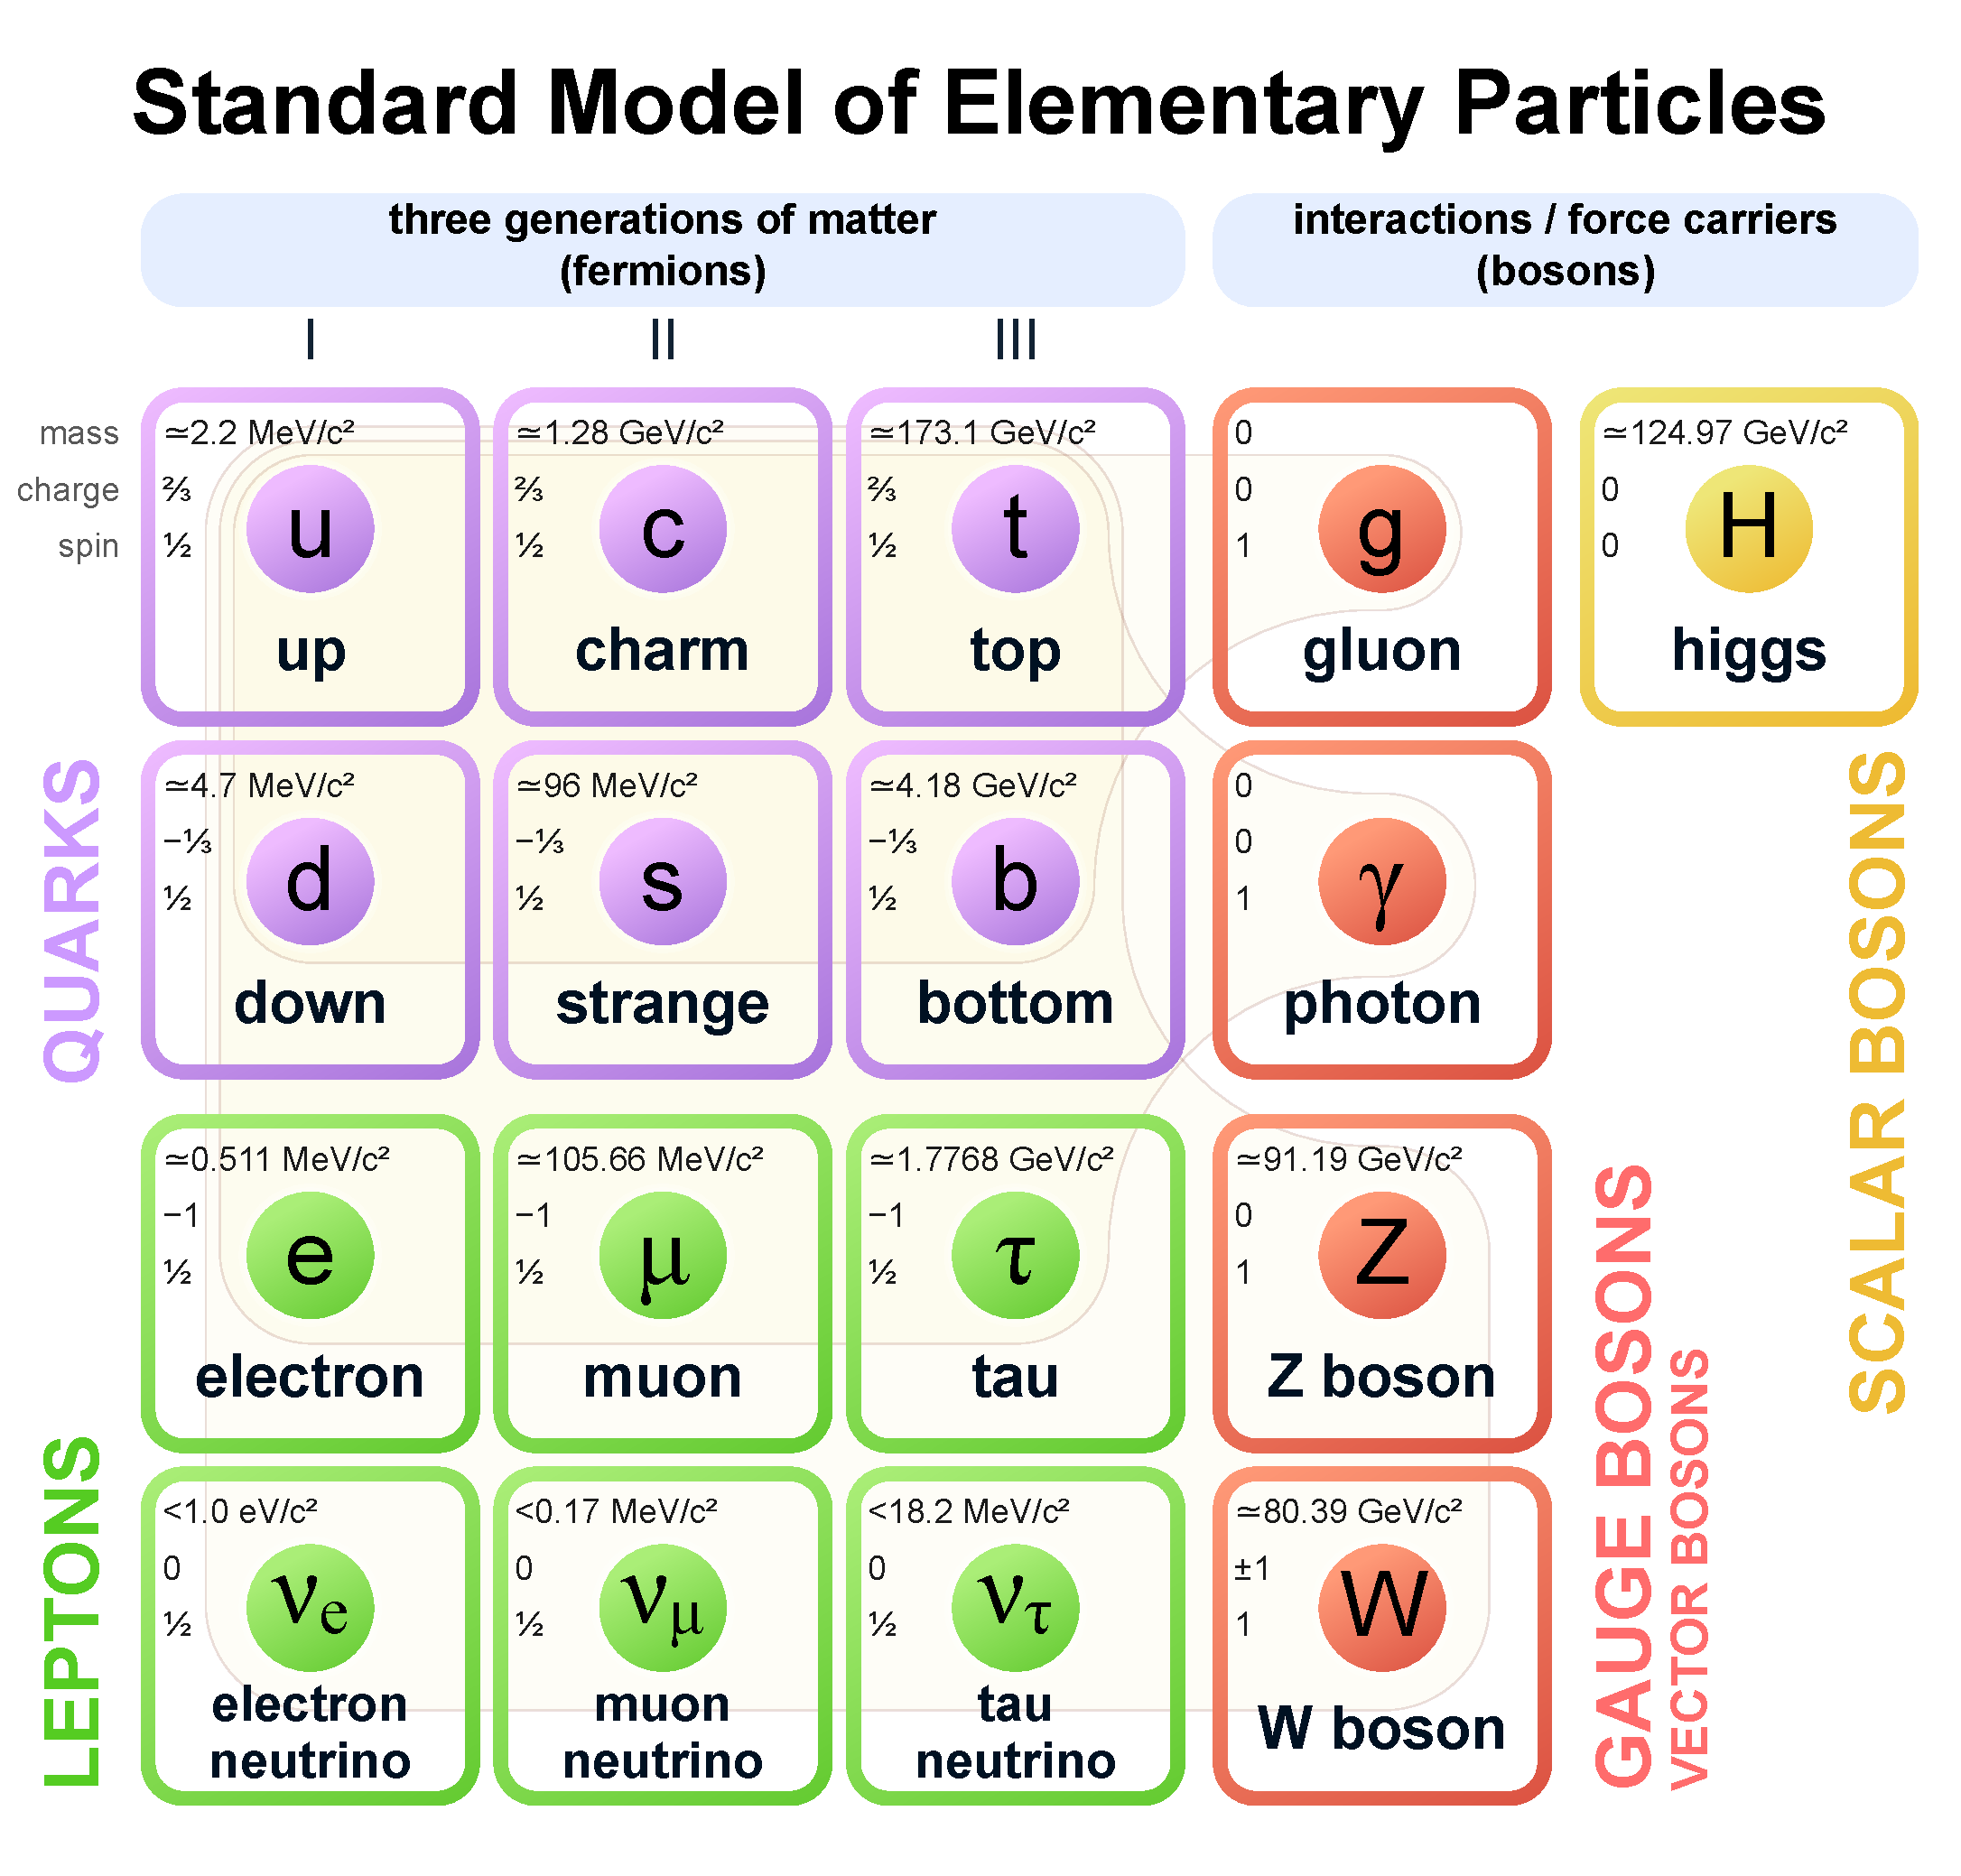
\includegraphics[width=0.9\textwidth]{fig/standard_model.pdf}
    \caption[The Standard Model of particle physics]{
        The Standard Model of particle physics arranged in a table with the fermions placed in the left three columns (one per generation) and the bosons in the right two columns.
    }
    \label{fig:standard_model}
\end{figure}

\subsection{Feynman diagrams}
Fortunately, there is way to encode essential Standard Model calculations in a simple drawings, so-called ``Feynman diagrams,'' which, consequently, help experimentalists keep track of physically allowed processes. 
In these pictures, time flows from left to right, while space is abstractly represented on the vertical axis\footnotemark{}. 
\footnotetext{In some dark corners of the physics community, these axes are switched, but this dissertation will not deviate from the configuration described here.}
The fundamental particles are represented by lines, and the intersections of three or four of these lines (Fig.~\ref{fig:sm_vertices}) represent interactions between the corresponding particles, so at least one of them must be a boson. 
For example, an electron emitting a photon (Fig.~\ref{fig:e_to_ge}) is represented by an electron coming in from the left, then turning into a photon and an electron leaving the picture to the right. 
This same vertex can be rotated clockwise, such that it instead depicts the annihilation of an electron and positron into a photon (Fig.~\ref{fig:ee_to_g})---one of the electrons had to be replaced with its anti-particle (a positron) to conserve charge. 
Rotating it again, we see that it now represents an electron absorbing a photon (Fig.~\ref{fig:eg_to_e}). 
These vertices act as building blocks that can be rotated and fit together according to a set of rules that correspond to real physical laws. 
Thus, any fundamental physical process (e.g. Fig.~\ref{fig:beta_decay}) can be represented with a Feynman diagram. 
Feynman diagrams are not only a visual aid for remembering which processes are allowed, however, for they also encode precise calculations about that process which can, importantly, be verified by experiment.

\begin{figure}[htb]
    \centering
    \subfloat[]{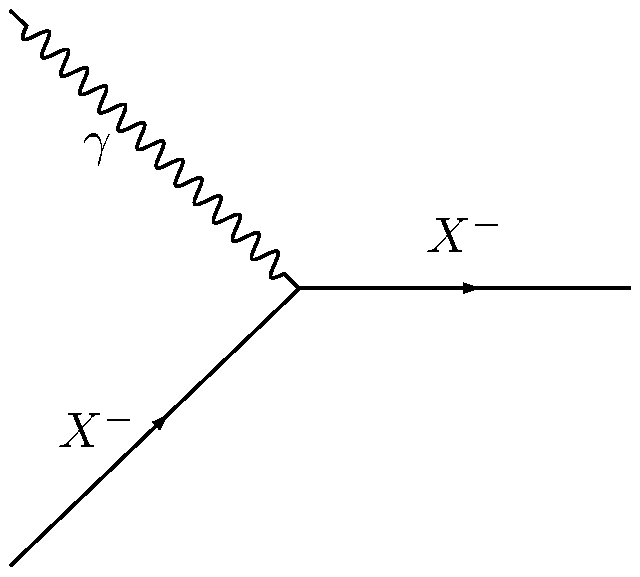
\includegraphics[width=0.2\textwidth]{fig/feynman/vertices/qed_vertex_2.pdf}\label{fig:qed1}}\qquad
    \subfloat[]{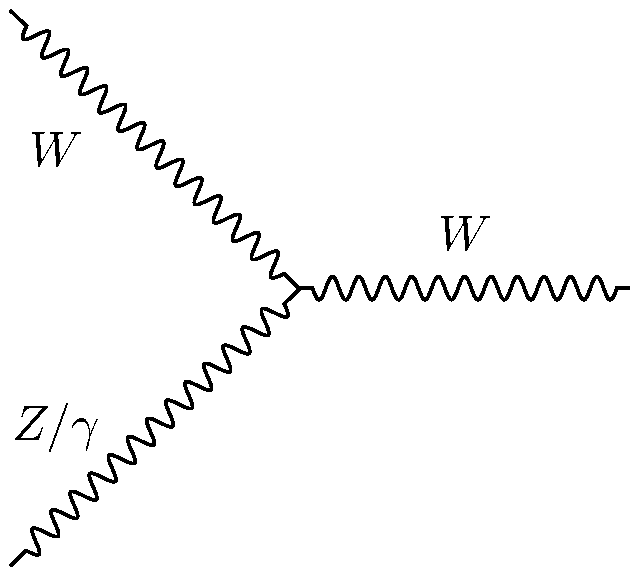
\includegraphics[width=0.2\textwidth]{fig/feynman/vertices/ewk_vertex_WWZ.pdf}\label{fig:ewk1}}\qquad
    \subfloat[]{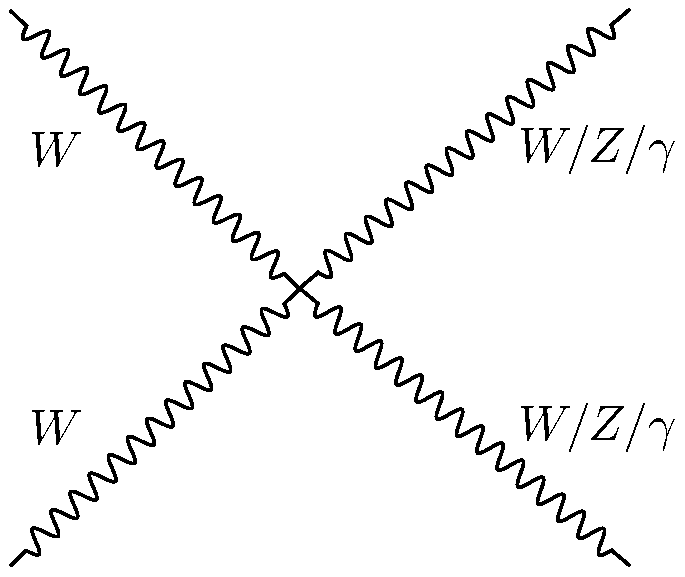
\includegraphics[width=0.2\textwidth]{fig/feynman/vertices/ewk_vertex_VVVV.pdf}\label{fig:ewk2}}\\
    \subfloat[]{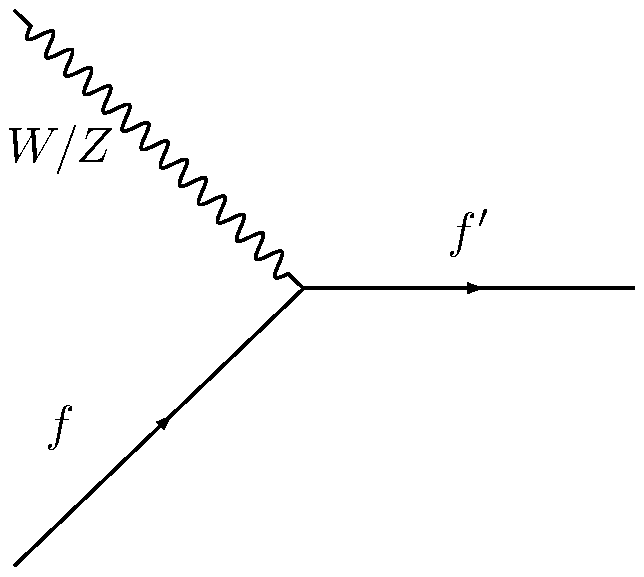
\includegraphics[width=0.2\textwidth]{fig/feynman/vertices/ewk_vertex_Vff.pdf}\label{fig:weak}}\qquad
    \subfloat[]{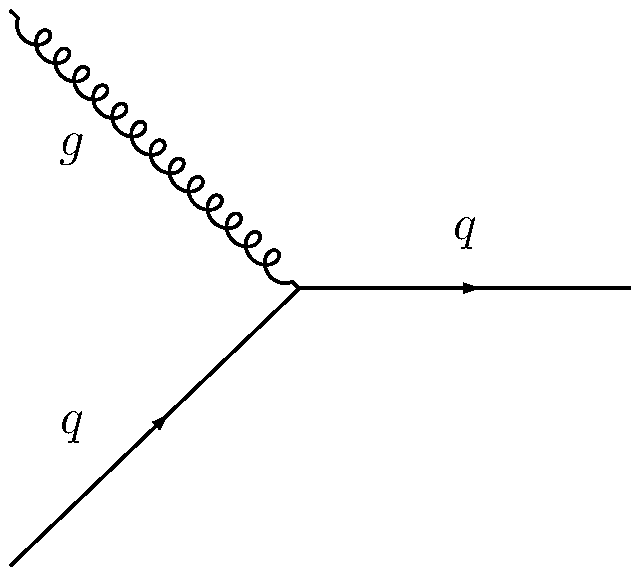
\includegraphics[width=0.2\textwidth]{fig/feynman/vertices/qcd_vertex_gqq.pdf}\label{fig:qcd1}}\qquad
    \subfloat[]{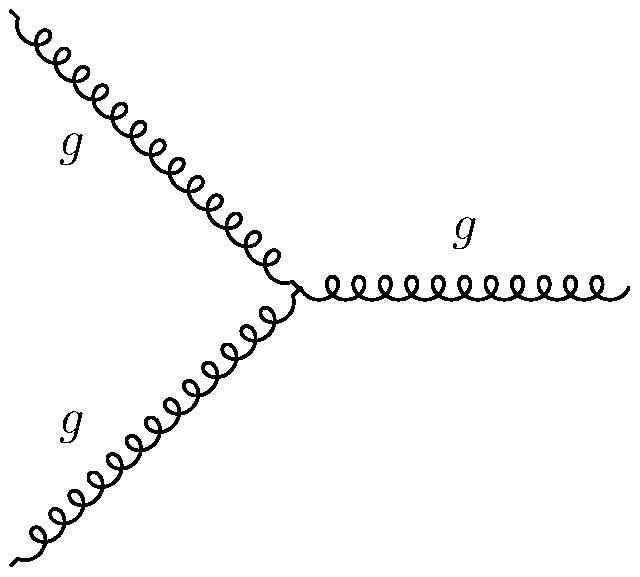
\includegraphics[width=0.2\textwidth]{fig/feynman/vertices/qcd_vertex_ggg.pdf}\label{fig:qcd2}}\\
    \subfloat[]{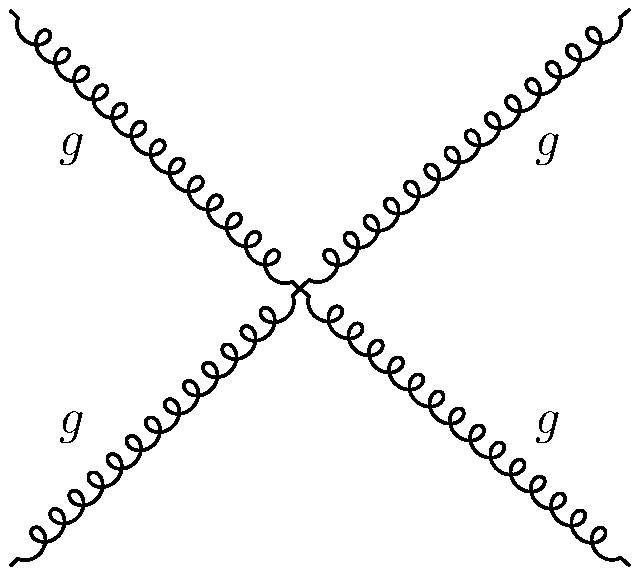
\includegraphics[width=0.2\textwidth]{fig/feynman/vertices/qcd_vertex_gggg.pdf}\label{fig:qcd3}}\qquad
    \subfloat[]{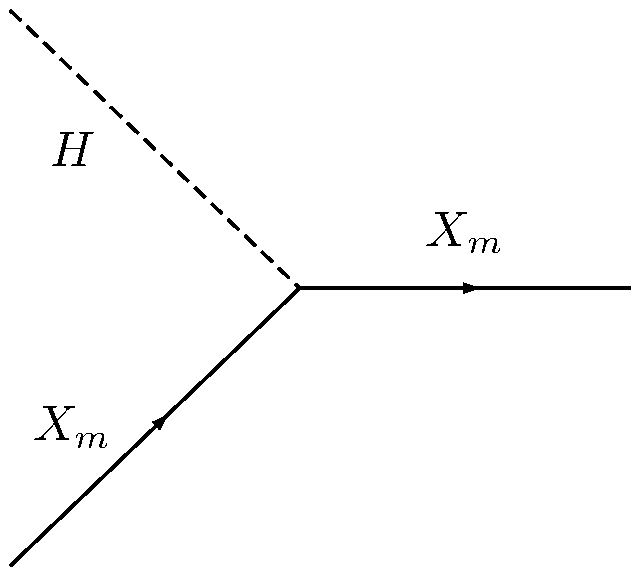
\includegraphics[width=0.2\textwidth]{fig/feynman/vertices/hig_vertex_HXX.pdf}\label{fig:hig1}}\qquad
    \subfloat[]{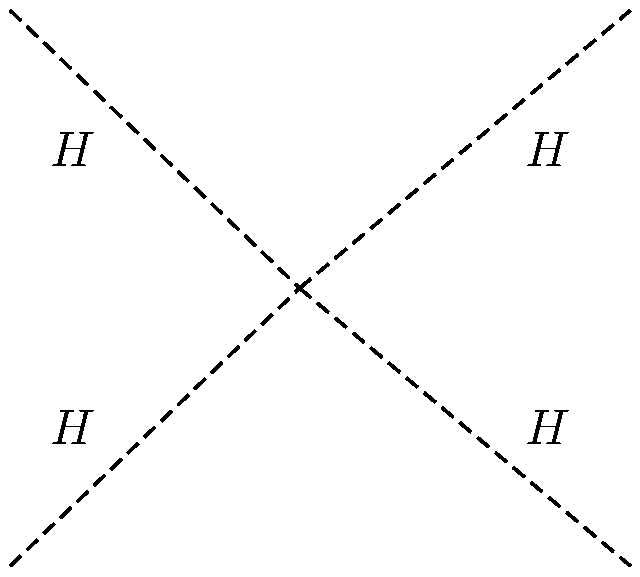
\includegraphics[width=0.2\textwidth]{fig/feynman/vertices/hig_vertex_HHHH.pdf}\label{fig:hig2}}
    \caption[The fundamental vertices in the Standard Model]{
        The fundamental vertices in the Standard Model. 
        From left to right, top to bottom: 
        (a) electromagnetic; (b), (c) electroweak; (d) weak; (e), (f), (g) strong; (h), (i) Higgs. 
    }
    \label{fig:sm_vertices}
\end{figure}

\begin{figure}[htb]
    \centering
    \subfloat[$\Pep+\Pem\to\PGg$]{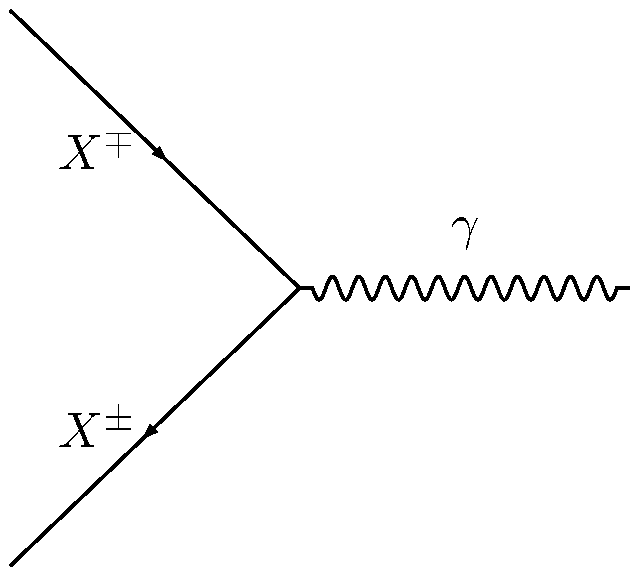
\includegraphics[width=0.25\textwidth]{fig/feynman/vertices/qed_vertex_1.pdf}\label{fig:ee_to_g}}\quad
    \subfloat[$\Pem+\PGg\to\Pem$]{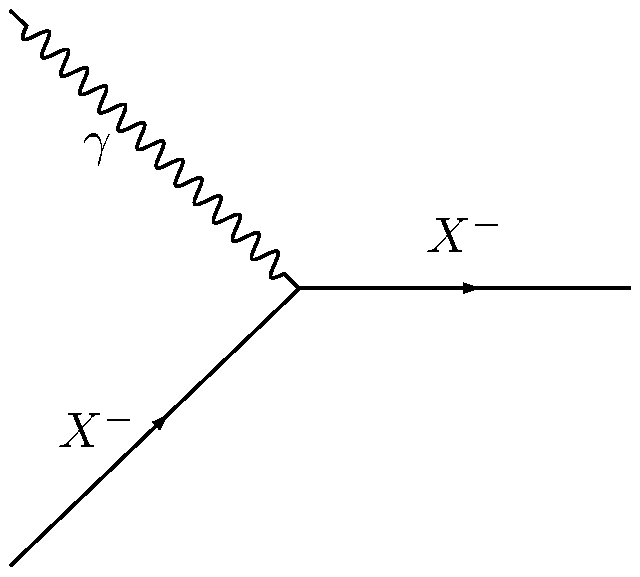
\includegraphics[width=0.25\textwidth]{fig/feynman/vertices/qed_vertex_2.pdf}\label{fig:eg_to_e}}\quad
    \subfloat[$\Pem\to\PGg+\Pem$]{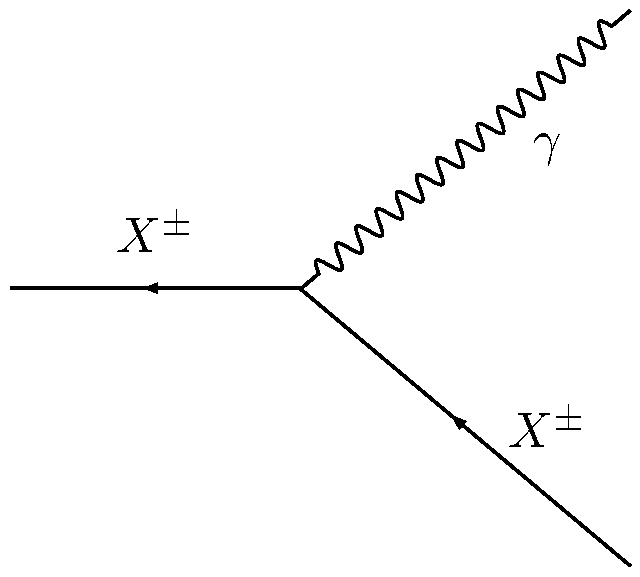
\includegraphics[width=0.25\textwidth]{fig/feynman/vertices/qed_vertex_0.pdf}\label{fig:e_to_ge}}
    \caption[Different versions of the QED vertex]{
        Rotations of the QED vertex, (a) an electron and positron annihilating and producing a photon, (b) an electron absorbing a photon, and showing (c) an electron emitting a photon.
    }
    \label{fig:qed_rotations}
\end{figure}

\begin{figure}[htb]
    \centering
    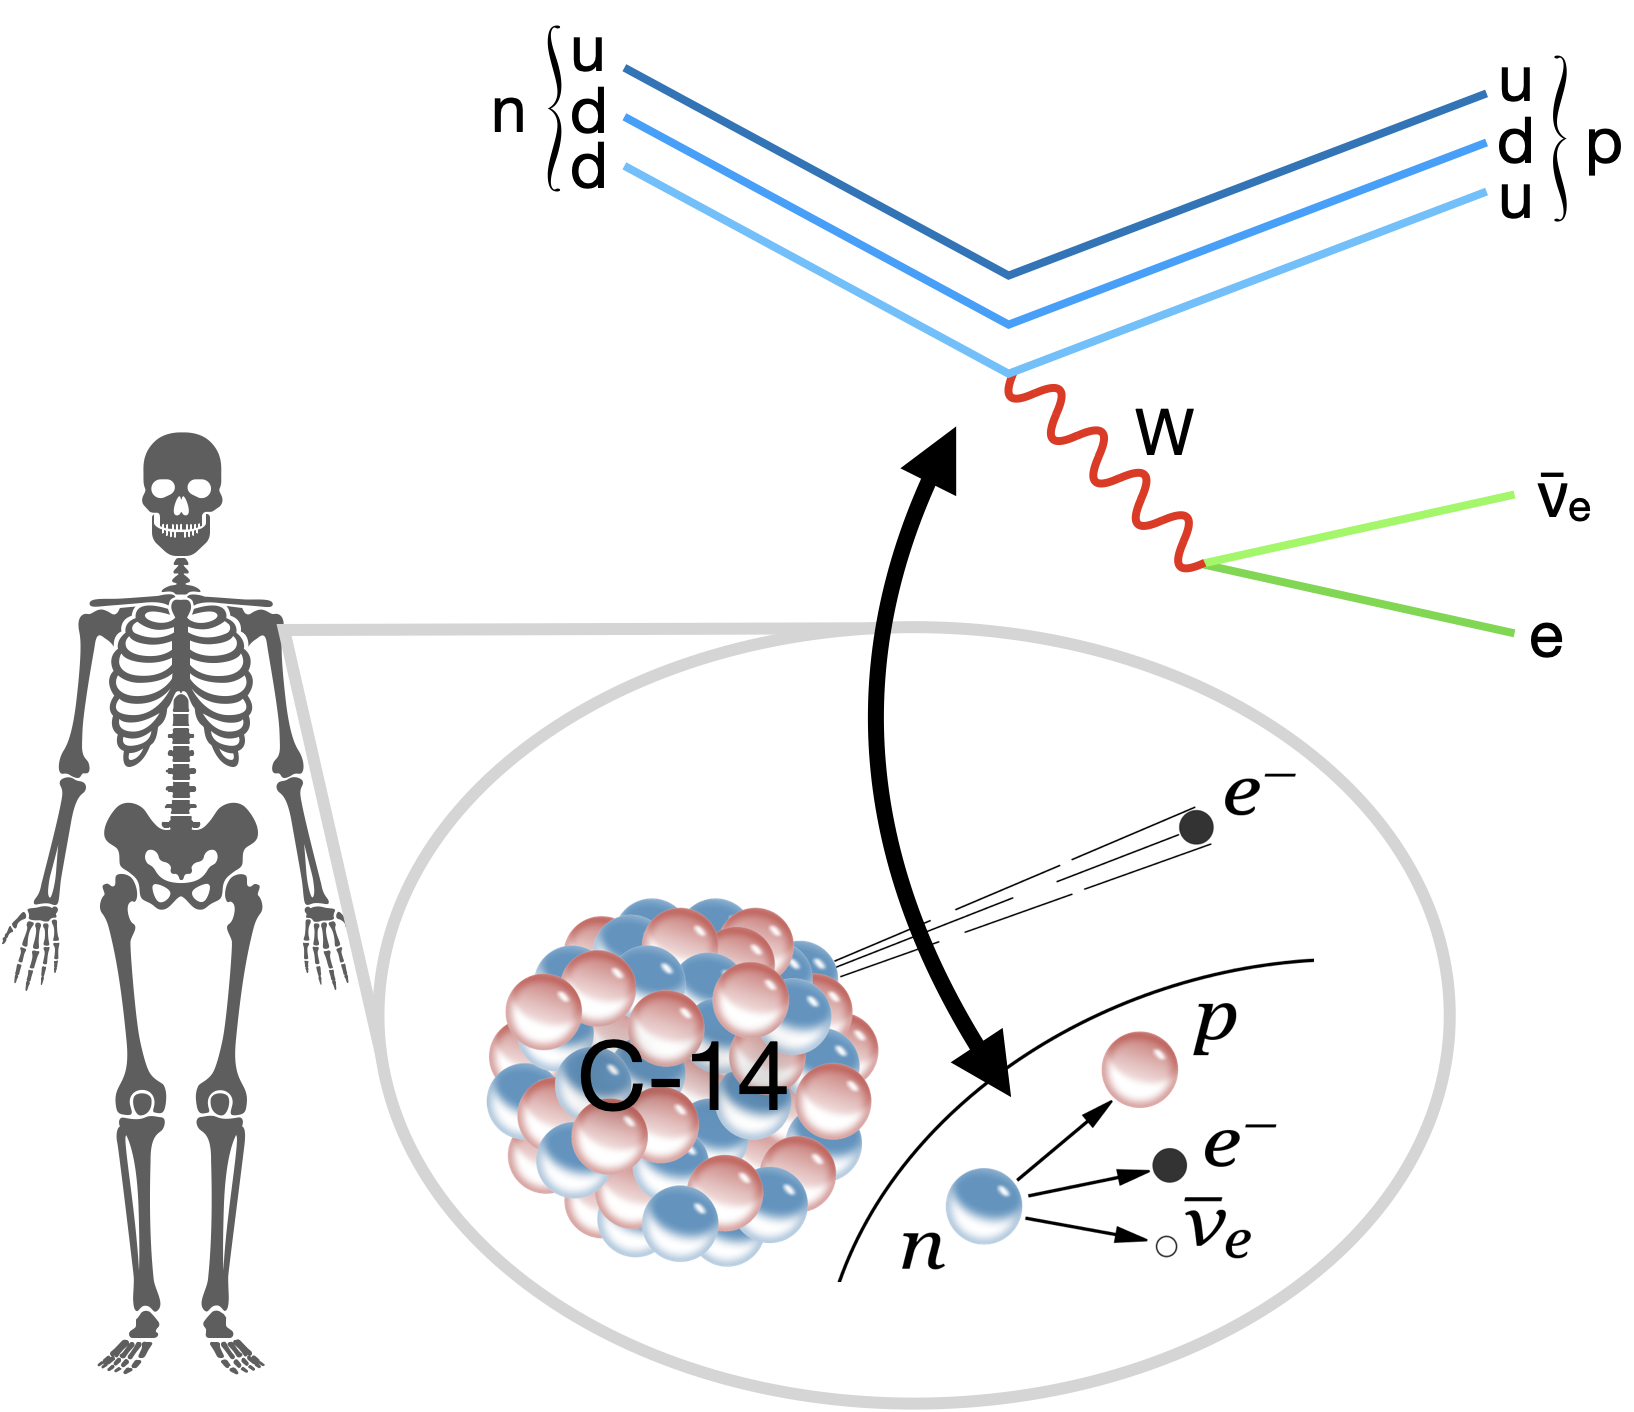
\includegraphics[width=0.45\textwidth]{fig/feynman/beta_decay.png}
    \caption{
        Feynman diagram for beta decay, which is mechanism behind the radioactive decay of certain elements. 
    }
    \label{fig:beta_decay}
\end{figure}

\subsection{Cross sections}
Consider two electrons barrelling towards each other with some velocity. 
In the classical picture, the electrons glance off one another and fly off to infinity at some angle to their original trajectories---like two errant ice skaters. 
This can be represented as a Feynman diagram (Fig.~\ref{fig:ee_scattering}) which is assembled from two EM vertices. 
Again, time flows from left to right, showing the two electrons entering, then the exchange of a photon, followed by the two electrons leaving, much like the classical picture. 
Now, suppose we construct two beams of electrons, aim them at each other, then turn them on (preferably after we leave the room). 
In this scenario, we may well want to know the probability that the two electrons will bounce off hach other (``scatter''). 
This probability is called the ``cross section,'' because it is mathematically similar to the classical picture\footnotemark{}, where we would compute the cross-sectional area presented to either of the colliding objects. 
\footnotetext{
    In fact, the answer to this question is expressed in the units of ``barns,'' literally as in ``hitting the broad side of a barn,'' coined by Manhattan Project scientists during World War II. % citatin needed
}
Indeed, one of the most important features of QFT is the ability to compute the cross section for scattering two electrons off of each other, as in this case, or any other interactions between particles. 
Feynman diagrams beautifully encode the complex mathematics at work here: each line and every vertex (where three lines meet) correspond a term in the calculation. 
For the electron-electron scattering example, this would look like
\begin{equation}
    \sigma = \langle|\mathcal{M}|^2\rangle = \frac{2g_e^4}{(p_1 \cdot p_3)^2(p_1 \cdot p_4)^2[(p_1 \cdot p_2)^4 + (p_1 \cdot p_3)^4 + (p_1 \cdot p_4)^4]}
\end{equation}
where $\sigma$ is the cross section, $p_1$ and $p_2$ are the four-momenta of the incoming electrons, $p_3, p_4$ are the four-momenta of the outgoing electrons, and $g_e$ is the EM coupling constant. 
This exercise, and the compact answer above, serves to demonstrate the sheer complexity of QFT calculations. 
Many details were left out beyond the computation itself (which is already a glaring omission), including details surrounding the spin of the electron, the definition of spin, the defition of four-momentum (and special relativity), and so on. 
Those details, and much more, can be found in the illustrious textbook from which this entire example was borrowed~\cite{GriffithsParticle}. 
Moreover, this feature of QFT---the ability to compute cross sections---is absolutely vital because it offers a way of testing the theory with observation: compute the probability that the event is expected to occur, then try to reproduce that event many times in the lab and see how many times it really happens. 

\begin{figure}[htb]
    \centering
    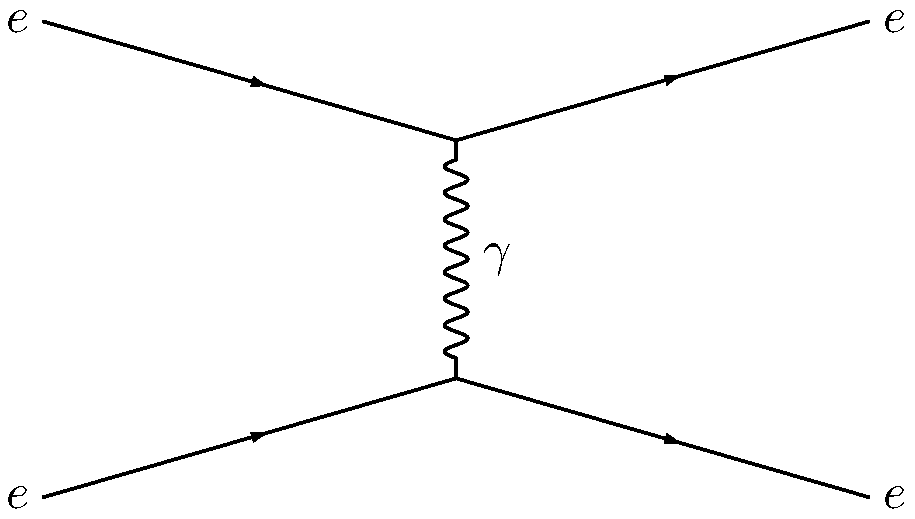
\includegraphics[width=0.6\textwidth]{fig/feynman/other/ee_scattering.pdf}
    \caption{
        Leading-order Feynman diagram for electron-electron scattering. 
    }
    \label{fig:ee_scattering}
\end{figure}

The validity of any model is a precarious condition: the model must exactly describe reality, else it is not a realization of the truth, but rather only approximately---or worse, accidentally---correct. 
That is, \textit{every} SM cross section value must be accurate for the validity of the model to hold. 
And so generations of physicists have made dilligent, and highly accurate, measurements of a dozens of cross sections---spanning orders of magnitude of rarity. 
Tabulated in grand tables (Fig.~\ref{fig:cms_xsecs} and \ref{fig:atlas_xsecs}), it is evident that the Standard Model has so far withstood every test derived from CMS data and ATLAS data. 
This is an incredible feat: a ``simple'' model seems to describe subatomic physics, which drove the creation of the universe and continues to drive the mechanics of everything, with incredible accuracy. 
Lingering beyond these shining trophies, however, are a number of glaring inconsistencies and enormous missing pieces. 
In other words, we know with certainty that the Standard Model is not complete, and that much more work is needed to complete it. 
We will focus in this dissertation on questions around the Higgs boson. 
However, we will also mention some additional open questions to illustrate the magnitude of the problem ahead for future particle physicists. 

\begin{figure}[htb]
    \centering
    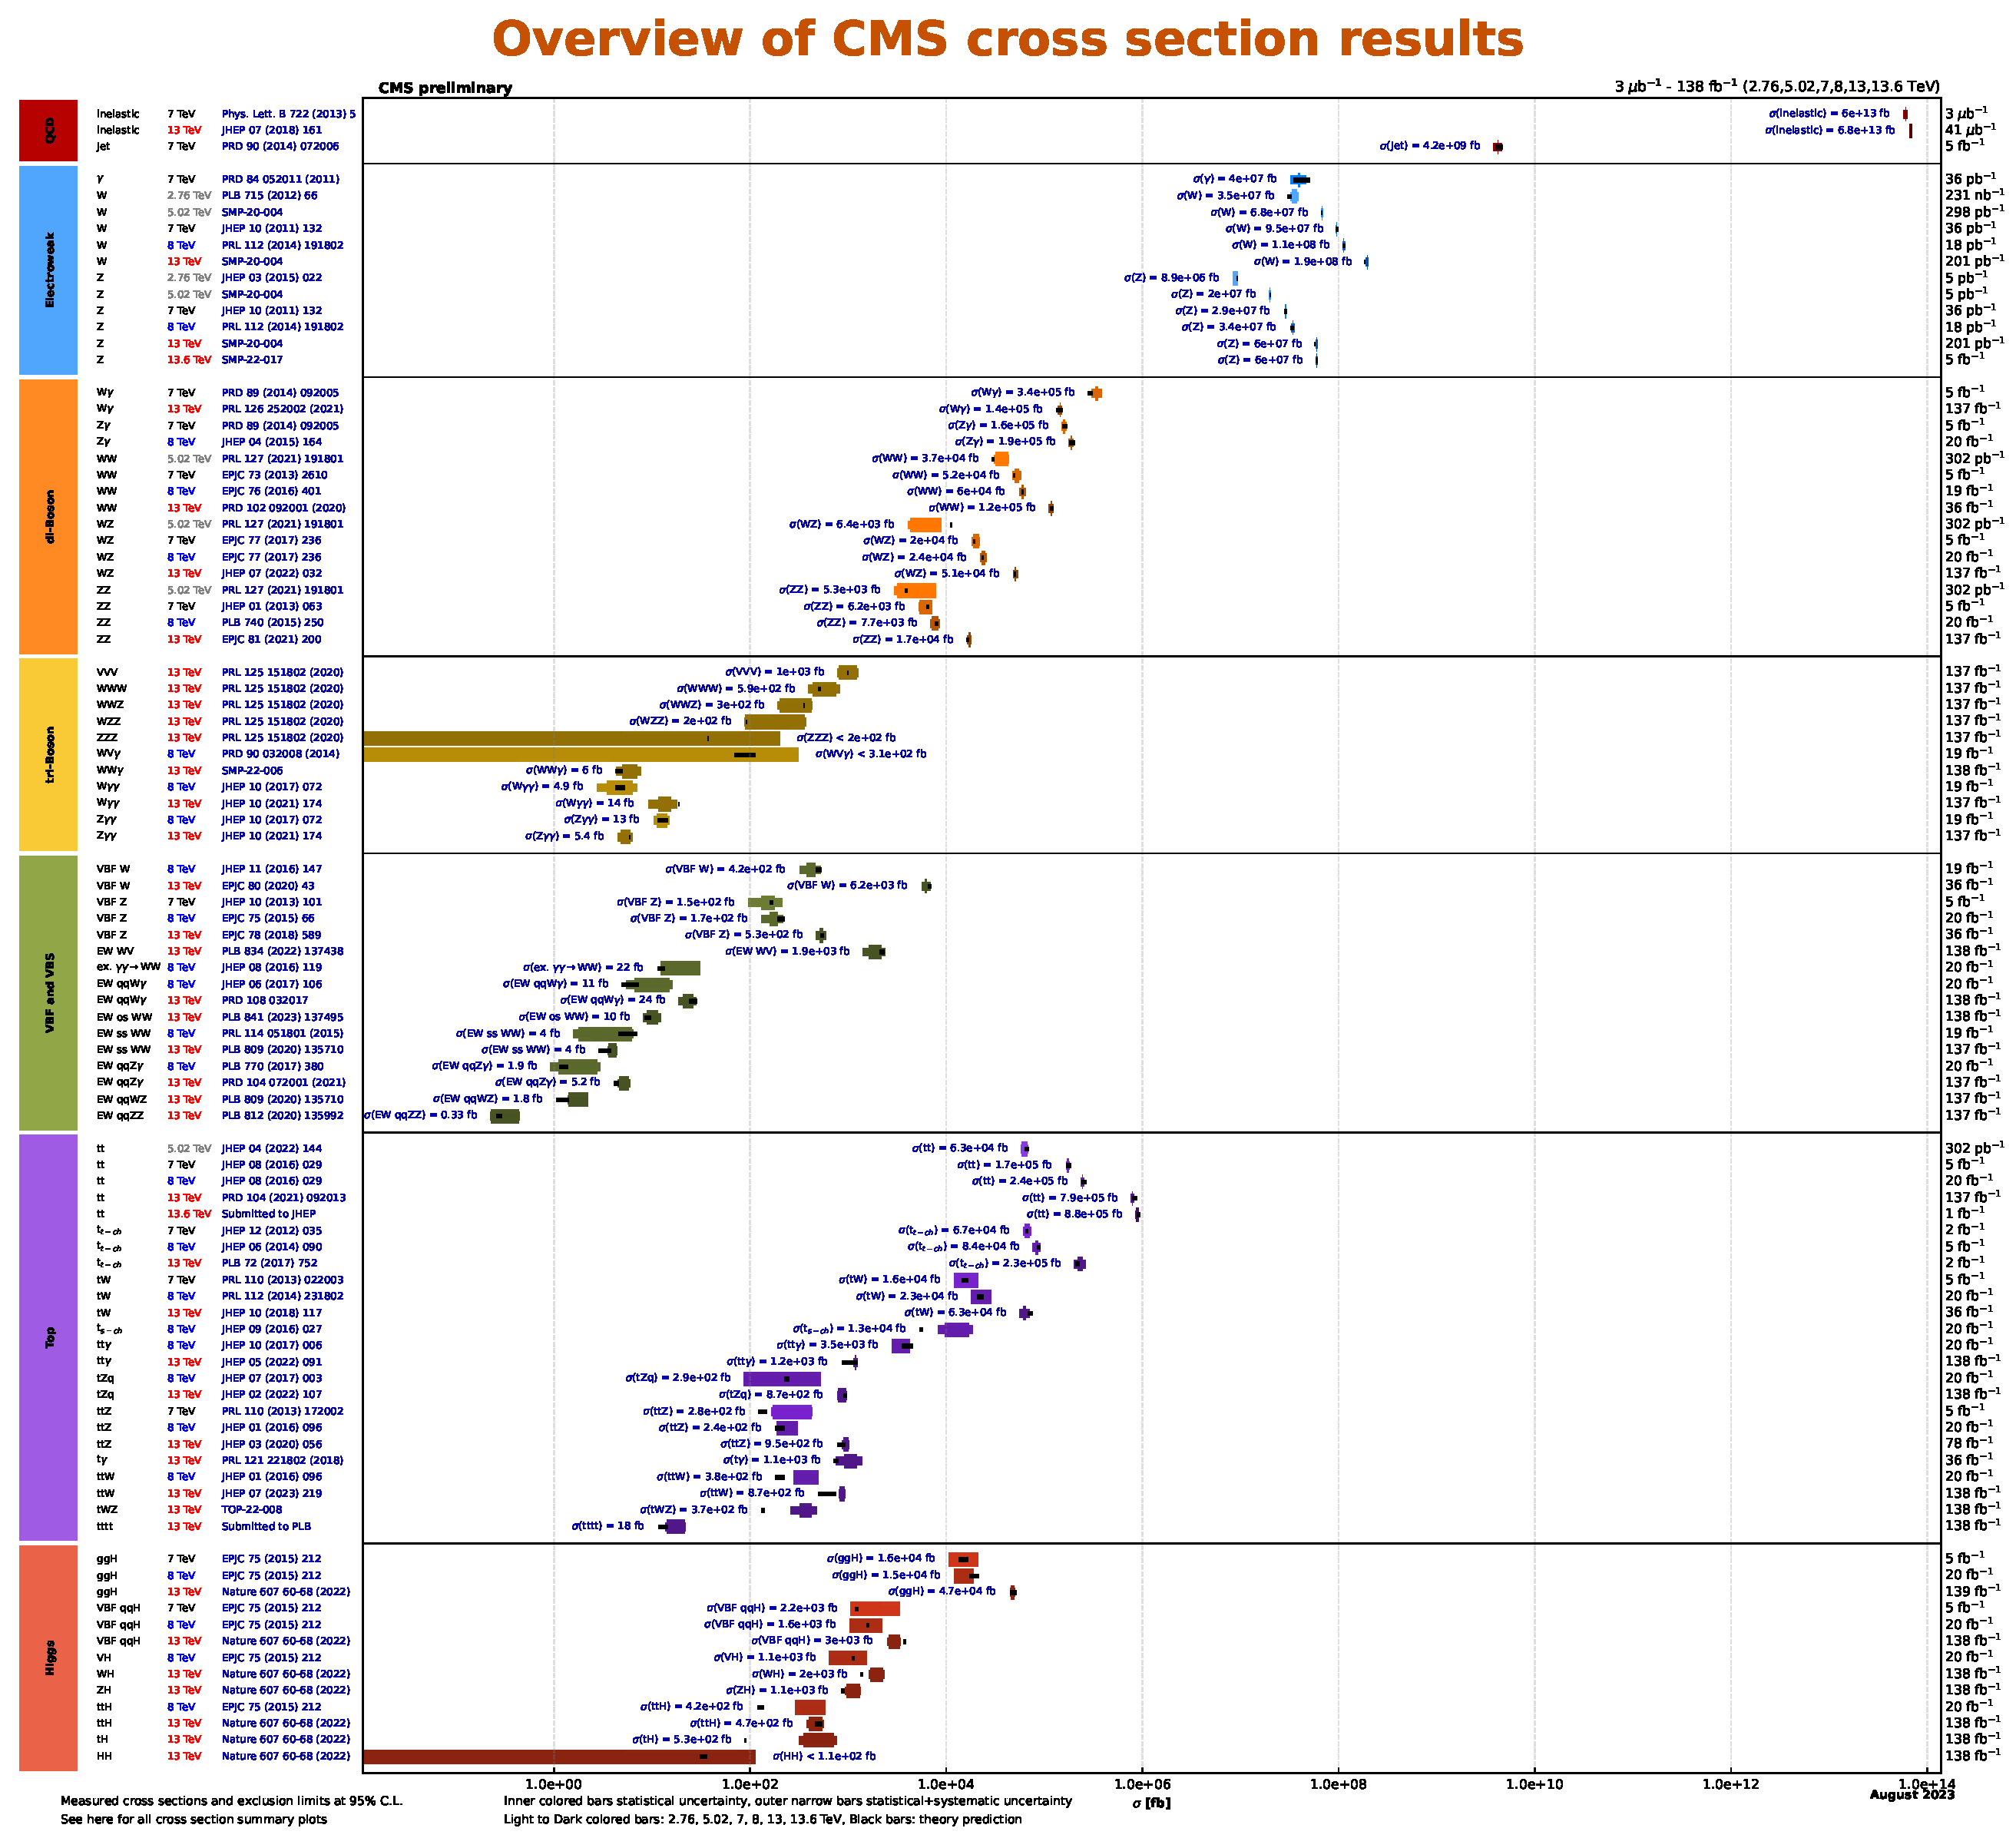
\includegraphics[width=0.95\textwidth]{fig/cms/cms_xsecs_2023.pdf}
    \caption[The totality of the cross section measurements performed with data from the CMS Experiment]{
        The totality of the cross section measurements performed with data from the CMS Experiment compared to the Standard Model predictions, from Ref.~\cite{CMSXSecs}. 
        Precise agreement with the Standard Model can be seen across several orders of magnitude, representing the triumph of the model across decades of experimental scrutiny. 
    }
    \label{fig:cms_xsecs}
\end{figure}

\begin{figure}[htb]
    \centering
    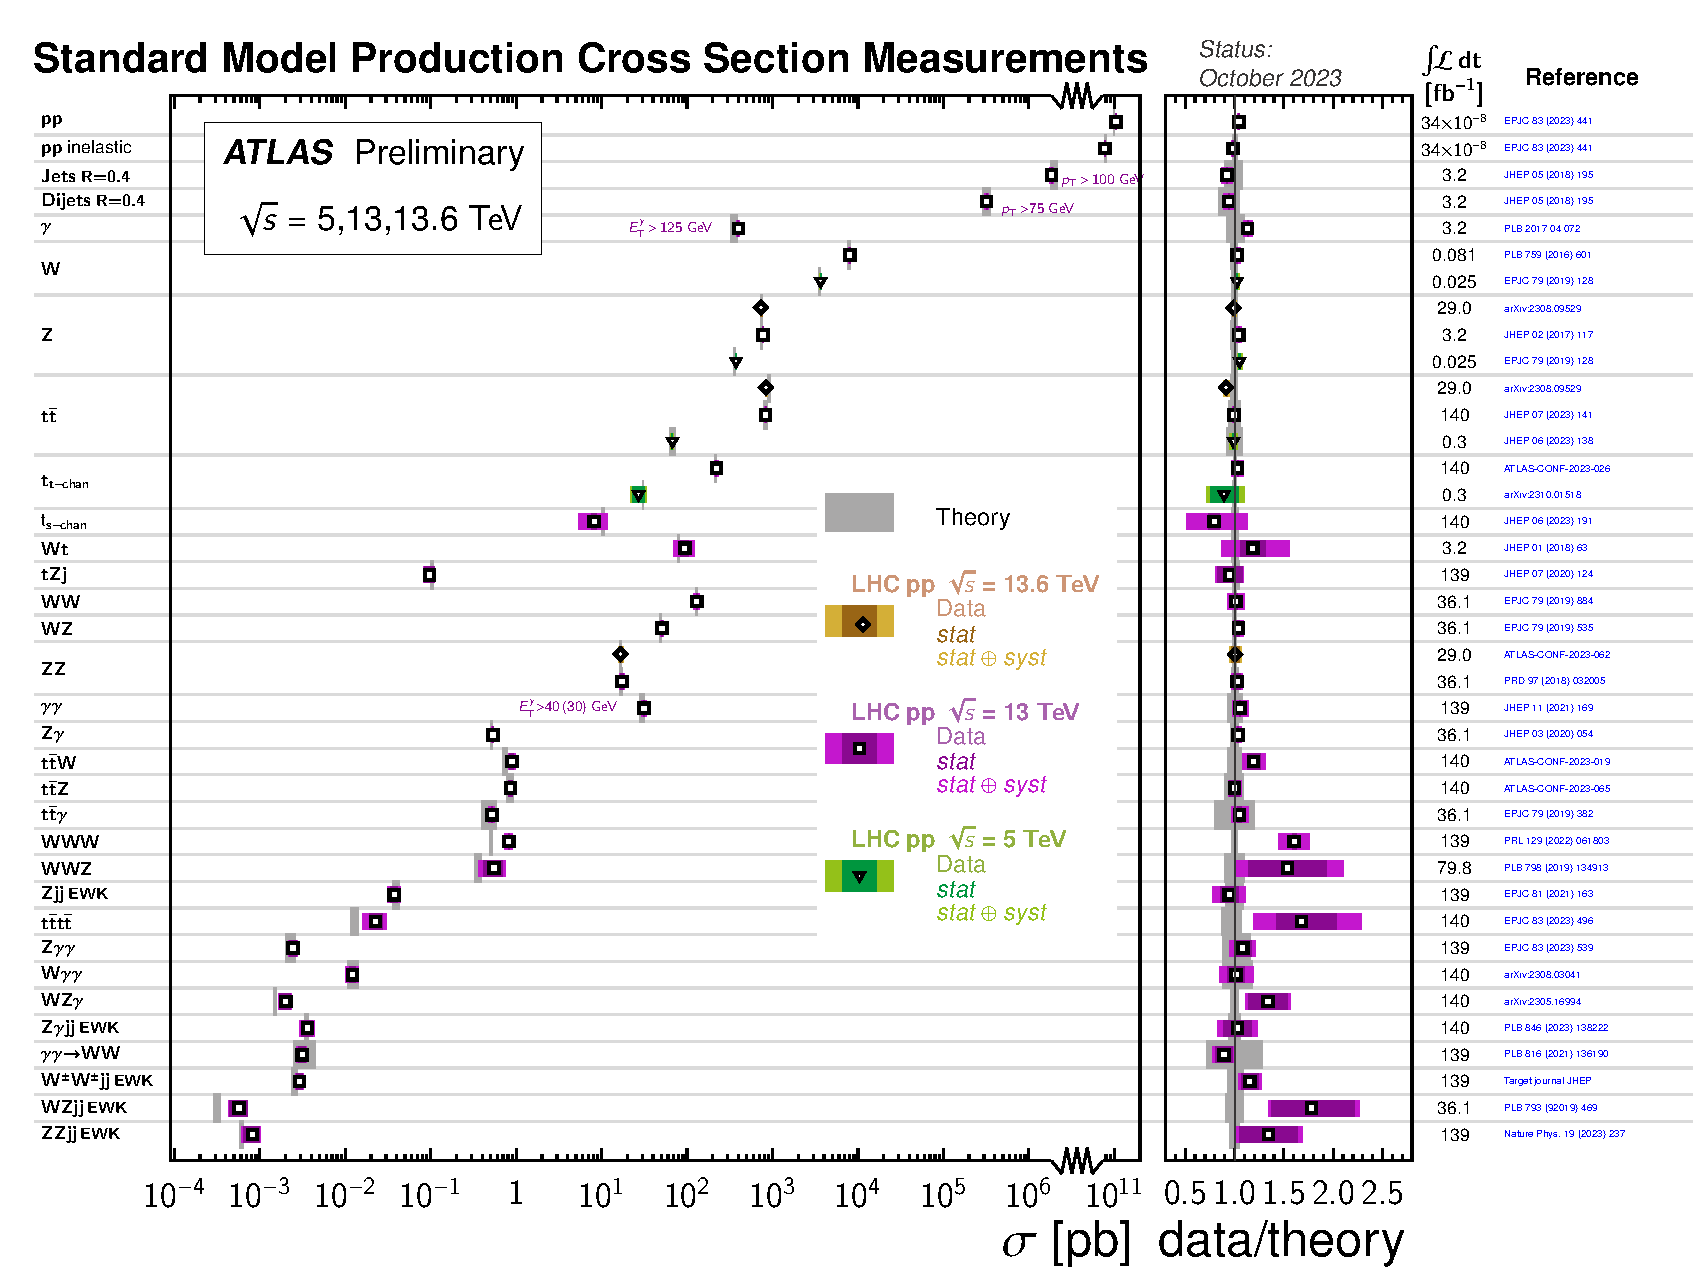
\includegraphics[width=0.95\textwidth]{fig/atlas/atlas_xsecs_2023.pdf}
    \caption[A selection of cross section measurements performed with data from the ATLAS Experiment]{
        A selection of cross section measurements performed with data from the ATLAS Experiment compared to the Standard Model predictions, from Ref.~\cite{ATL-PHYS-PUB-2023-039}. 
        Precise agreement with the Standard Model can be seen across several orders of magnitude, representing the triumph of the model across decades of experimental scrutiny. 
    }
    \label{fig:atlas_xsecs}
\end{figure}

\subsection{The Higgs boson}\label{sec:higgs}
Because we swore to steer away from the details of QFT, we cannot define the Higgs boson and Higgs mechanism completely. 
For this, we are better served by a primer by Griffiths~\cite{GriffithsParticle}, followed by the standard QFT textbooks~\cite{SrednickiQFT, PeskinSchroederQFT}, and finally the original papers on the subject~\cite{EnglertBroutPRL, HiggsPhysLett, HiggsPRL, GuralnikHagenKibblePRL}. 
Without these prerequisites, it suffices to say that the idea of the Higgs boson is deeply based in Lagrangian mechanics. 
Originally derived for classical systems---an arrow in flight, a planet in motion, a ball on a ramp---an appropriately written ``Lagrangian,'' a mathematical object, together with the Euler-Lagrange equation can reproduce the mathematical description of the dynamics of a given system---the position of the arrow, planets, or ball as a function of time. 
The Lagrangian $L$ is a simple function of the energies in a classical mechanics:
\begin{equation}
    L = \underbrace{\frac{1}{2}m\dot{x}^2}_\text{kinetic energy} - \underbrace{U(x)}_{\substack{\text{potential} \\ \text{energy}}}
\end{equation}
where $x$, really $x(t)$, is the position of some physical object in one direction as a function of time and $\dot{x}$ is shorthand for the derivative of x with respect to time ($\frac{d}{dt}$), or the velocity. 
By plugging $L$ into the Euler-Lagrange equations, 
\begin{equation}
    \frac{d}{dt}\bigg(\frac{\partial L}{\partial\dot{x}}\bigg) = \frac{\partial L}{\partial x}
\end{equation}
we can solve for $x(t)$ with some algebra and calculus, trivializing some of even the most challenging undergraduate classical mechanics problems. 

In particle physics, we promote $x(t)$ to a field\footnotemark{} $\phi$, which is a function of space and time $\phi(x, y, z, t)$, and $L$ to $\mathcal{L}$, a Lagrangian \textit{density}.
\footnotetext{Fields are used here in a quantum context (scalar fields in particular) but there are many classical examples: the temperature of a room, the height of the sea, the strength of a magnetic field, these are quantities that may be different at every position in space and may also vary in time.}
Our interest in these abstract fields is well-motivated in QFT, where a field $\phi(x,y,z,t)$ with certain properties corresponds to an observable particle with those same properties. 
For example, the Lagrangian 
\begin{equation}
    \mathcal{L} = \underbrace{\frac{1}{2}(\partial_\mu\phi)(\partial^\mu\phi)}_{\text{kinetic term}} - \underbrace{\frac{1}{2}\big(\frac{mc}{\hbar}\big)^2}_\text{mass term}
\end{equation}
represents a spin-0 particle with mass $m$. 
As in classical machanics, plugging the appropriate Lagrangian density into the Euler-Lagrange equation yields the precise descriptions of the dynamics of fundamental particles. 

The Higgs mechanism arises when we try to write down a Lagrangian density $\mathcal{L}$ that accounts for the existence of the \PW and \PZ bosons. 
In doing so, we find that we must demand that $\mathcal{L}$ does not change under certain transformations of the fields $\phi$, which, at face value, equates to demanding that the field is massless---the finer details here are far beyond the scope of this dissertation. 
This is a problem because the \PW and \PZ bosons are verifiably not massless. 
However, by introducing two scalar fields---corresponding to the Higgs boson and Goldstone boson---and massaging the mathematics, a mass term emerges for the \PW and \PZ bosons. 
The Goldstone boson does not correspond to a real particle, but instead services the mathematics\footnotemark{} and disappears under a specific transformation. 
\footnotetext{For example, it accounts for the fact that there are three bosons that carry the weak force ($\PW^{+}$, $\PW^{-}$, \PZ).} 
The Higgs \textit{mechanism} itself refers to the appearance of the \PW and \PZ boson masses, as well as the fermion masses through different interactions~\cite{Weinberg:1967tq, Nambu:1961fr}. 

Beyond the blackboard, the Higgs boson gives us a picture of how the universe came to be: in the first moments of time, the universe cooled, allowing the Higgs field saturated all of space, and the fundamental particles were thereby endowed with mass by the Higgs mechanism. 
Thus, rather than fly off to infinity at the speed of light, they formed atoms, and the universe as we know it bloomed.  
The Higgs boson is therefore essential to the origin and continued existence of the known universe---in fact, if the Higgs field were to spontaneously dissappear, the entire universe would evaporate in a nanosecond~\cite{P5Report}. 
It is also, however, a key to understanding the universe's distant future~\cite{Bass2021}: will the universe collapse or explode or something else entirely? 
We shall spare ourselves of existential crisis and instead simply appreciate the specific importance of the Higgs boson. 
While every piece of the Standard Model is important, like links in a chain, the Higgs boson is also one of the less well-understood particles, so further study of this latest addition to the Standard Model could shed crucial light on the many open questions in particle physics. 

\section{Selected open questions}\label{sec:open_questions}
\subsection{What is dark matter?}
In the 1970s, Vera Rubin, among others, was making careful observations of the rate at which distant galaxies spin on their axes~\cite{VeraRubin}.  
By also recording the light emitted by each galaxy, she could estimate the distribution of mass within it, and therefore calculate the expected rotational velocity due to the gravitational pull of a galaxy's constituents. 
The observation and prediction did not align, leading us to believe that there is some ``dark'' matter that we cannot see and is therefore missing from our calculations. 
In fact, based on the observable mass in a galaxy, we would expect it to fly apart~\cite{GalaxyDM}. 
Today, as we probe the subatomic world at unprecedented scales, we have yet to observe any new particle that might be the right candidate for dark matter---really, we have yet to observe any new particle whatsoever. 
Dark matter is therefore an enormous missing piece---26\% of the universe~\cite{PlanckDM}---in the Standard Model.

\subsection{What is dark energy?}
Cosmology yields yet another missing piece in the Standard Model, but at a completely different scale than dark matter. 
Measurements of the cosmic microwave background (CMB) radiation, light from the early universe, and of distant galaxies shows clear indication that the universe is expanding: all of this light has been stretched out, with visible light appearing an eerie red. % TODO: citation needed
But what is driving this expansion? 
With no known answer to this question, we have yet another invisible quantity---this time, a ``dark'' energy that constitutes 69\% of the universe~\cite{PlanckDM}---as a placeholder.

\subsection{What is the true nature of the Higgs boson?}
The Higgs boson holds many secrets yet to be uncovered, despite being discovered over a decade before the publication of this dissertation. 
It is one of the central physics targets of the LHC for the coming decades, and only a few of the most interesting questions are summarized here:
\begin{itemize}
    \item{
        \textit{Is the Higgs boson really a fundamental particle?}
        Pursuing an ever-reductive line of reasoning, it is important to always ask if a particle is in fact a composite particle, rather than a fundamental one. 
        A number of theories that predict a composite Higgs boson exist, e.g. Refs.~\cite{Kaplan:1983sm, Arkani-Hamed:2002ikv, Contino:2003ve}, and, if true, they may explain other open questions around the nature of the Higgs boson.
    }
    \item{
        \textit{Is there only one Higgs boson?}
        In a 2012 interview at CERN, only 6 months before the discovery of the Higgs boson, Murray Gell-Mann mused
        \begin{quote}
            As to there being one boson that results from this Higgs process, it's not quite so certain because there could be more than one... 
            and [CMS and ATLAS] might not be looking for it in the right way for that.
        \end{quote}
        Although only a single Higgs boson was discovered, the existence of others, e.g. Refs.~\cite{Branco:2011iw, Gunion:2005ja, Grzadkowski:2009bt}, could again answer other open questions around the nature of the Higgs boson.
    }
    \item{
        \textit{Why is the Higgs boson mass so small?}
        While nearly as heavy as the most massive SM particle, the top quark, the Higgs boson is not nearly as massive as it ``should'' be. 
        Corrections from heavier particles---even unknown ones---could make the Higgs boson over 16 orders of magnitude heavier, so some new physics should correct this somehow~\cite{Susskind:1978ms, tHooft:1979rat}.
    }
\end{itemize}
